\documentclass[informe,english]{plantilla}
\usepackage[T1]{fontenc}   % so { } show correctly in \texttt
\usepackage[background]{lst-shell}
\usepackage[background]{lst-c}
\usepackage[background]{lst-python}
\usepackage{graphicx}
\usepackage{amsmath}
\usepackage{amsfonts}
\usepackage{amssymb}
\usepackage{enumitem}
\usepackage{float}
\usepackage{textcomp}
\usepackage{algorithm}
\usepackage{algpseudocode}
\usepackage{xcolor}
\usepackage{booktabs}
\usepackage{pgfplots}
\pgfplotsset{compat=1.17}
\usetikzlibrary{positioning, shapes.geometric, arrows.meta, calc}

% Flowchart styles
\tikzset{
  fc/.style={font=\footnotesize, align=center},
  proc/.style={fc, rectangle, draw, fill=blue!6, text width=5.2cm, minimum height=0.65cm, inner sep=3pt},
  term/.style={fc, rectangle, rounded corners=6pt, draw, fill=gray!15, text width=5.2cm, minimum height=0.65cm, inner sep=3pt},
  dec/.style={fc, diamond, aspect=3.2, draw, fill=orange!12, inner sep=1.5pt},
  arr/.style={-{Stealth[length=2mm]}},
  lbl/.style={font=\scriptsize},
}

\title{Weather station system}
\assignatura{Internet of Things Connectivity}
\subtitle{Activity 2: LoRa-based communication with MQTT integration ---
  \textsf{Internet of Things Connectivity}}
\numpract{2}
\autor{Aarón Alcalá \and Marcos García \and Jaume Pulido \and Mikael Rodríguez}
\date{\today}

% Footer strings in English (the class writes them in Catalan by default)
\makeatletter
\ifoot[Report~\practno.~\@assignatura]{%
  \def\and{, }\@author. Report~\practno.~\@assignatura}
\ofoot[\pagemark]{\pagemark}
\makeatother

% custom commands
\newcommand{\tcmp}[1]{\textlangle #1\textrangle}
\providecommand{\todo}[1]{\textcolor{red}{\textbf{[TODO: #1]}}}

\lstset{
  style=lst-common,
  backgroundcolor=\color{upcblue!8!white},
  basicstyle=\ttfamily\footnotesize,
  breaklines=true,
  postbreak=\mbox{\textcolor{upcred}{$\hookrightarrow$}\space},
  captionpos=b,
  keywordstyle=\color{upcblue}\bfseries,
  aboveskip=5pt,
  belowskip=5pt,
}

\lstdefinestyle{arduino}{
    language=C++,
    basicstyle=\ttfamily\footnotesize,
    keywordstyle=\color{blue!70!black}\bfseries,
    commentstyle=\color{green!45!black}\itshape,
    stringstyle=\color{orange!80!black},
    numbers=left, numberstyle=\tiny\color{gray},
    frame=single, breaklines=true, showstringspaces=false,
    tabsize=4, captionpos=b
}

\begin{document}
\newpage

% =====================================================================
\section{Introduction}
\label{sec:intro}
% =====================================================================
This report documents Activity 2 of the Weather station system, which extends the MQTT chain of Activity 1 by introducing a LoRa link between two ESP32 boards: a transmitter (TX) node that reads the DHT11 sensor and sends the data over LoRa, and a receiver (RX) node that forwards what it receives to the Mosquitto broker over MQTT, so that the dashboard remains unchanged.

Two groups joined forces for this activity: Jaume Pulido and Mikael Rodríguez developed the TX node, including the DHT11 handling, and Aarón Alcalá and Marcos García developed the RX node, whose WiFi connection, MQTT publication and web frontend keep the structure of Activity 1.

% =====================================================================
\section{LoRa Configuration}
\label{sec:lora-config}
% =====================================================================

The configuration and communication logic are separated into different files. \texttt{LoRaConfig.h} defines the radio configuration structure, \texttt{config.h} contains the default radio parameters and pin assignments, and \texttt{LoRa\_IOT.h/.cpp} implement the communication interface (initialisation, transmission and reception) on top of the Arduino LoRa library. This allows the radio parameters to be changed without touching the application logic.

\subsection{Radio Parameters}
\label{sec:lora-params}

Table~\ref{tab:lora-params} summarises the parameters, which are passed to the initialisation function through the \texttt{LoRaConfig} structure.

\begin{table}[htbp]
    \centering
    \small
    \begin{tabular}{@{}llp{0.55\textwidth}@{}}
        \toprule
        \textbf{Parameter} & \textbf{Value} & \textbf{Rationale} \\
        \midrule
        Frequency        & 868~MHz  & European ISM band. \\
        Bandwidth        & 250~kHz  & Higher data rate than narrower bandwidths, suited to small periodic messages. \\
        Spreading factor & SF7      & Short time on air, enough range for the expected distances. \\
        Coding rate      & 4/5      & Forward error correction with minimal overhead. \\
        Sync word        & 0x12     & Filters packets from networks with a different sync word. \\
        Preamble         & 8 symbols & Packet detection and synchronisation with low overhead. \\
        CRC              & Enabled  & Detection of corrupted packets. \\
        \bottomrule
    \end{tabular}
    \caption{LoRa radio parameters shared by the TX and RX nodes.}
    \label{tab:lora-params}
\end{table}

The transmit power is also configurable and must comply with the regional regulations.

\subsection{Compatibility and Interference}
\label{sec:lora-software}

Both boards must use exactly the same frequency, bandwidth, spreading factor, coding rate and sync word, which is why these parameters are centralised in a single configuration shared by both nodes. The sync word reduces the chance of accepting packets from unrelated LoRa networks, but it does not prevent interference or collisions on the shared channel, and it provides neither encryption nor authentication. A GPIO interrupt on the radio signals the arrival of a packet to the main program without polling (Section~\ref{sec:rx}).

% =====================================================================
\section{TX node (\texttt{src/tx/main.cpp})}
\label{sec:tx}
% =====================================================================

The transmitter is the node placed at the weather station. It reads the DHT11 sensor periodically and sends each reading over LoRa to the receiver. 

It is built in its own PlatformIO environment (\texttt{env:tx}), which compiles only \texttt{src/tx/} through \texttt{build\_src\_filter}. The DHT11 is connected to GPIO~13 and a reading is sent every 5~s (\texttt{LORA\_SEND\_INTERVAL\_MS}).

\subsection{Initialisation}

In \texttt{setup()}, the node opens the serial port for debugging, starts the DHT11 driver and calls \texttt{LoRaIOT\_setup()} with the default \texttt{LoRaConfig}. This function starts the SPI bus on the pins of the on-board SX1276, calls \texttt{LoRa.begin()} with the carrier frequency, applies the parameters of Table~\ref{tab:lora-params} and the transmission power, and enables the CRC. If the radio does not respond, the program stops, since the node is useless without it.

\subsection{Main loop}

The main loop is summarised in Figure~\ref{fig:tx-flow}. First, the temperature and humidity are read from the DHT11. Then the node checks that both values are valid: if the driver returns \texttt{NaN} (for example, because the sensor was read too often or a wire is loose), nothing is sent and the reading is retried after 2~s, so invalid values never reach the receiver. Otherwise, the reading is formatted as a JSON object with one decimal, the resolution of the DHT11:
\begin{center}
    \texttt{\{"id":12,"temp":23.4,"hum":55.0\}}
\end{center}
The \texttt{id} field is a counter incremented on every iteration, which allows the receiver to detect lost or duplicated packets as gaps or repetitions in the sequence. JSON was chosen because the receiver can parse it directly with ArduinoJson, and the message stays far below the 255-byte limit of a LoRa packet. Finally, the message is sent with \texttt{LoRaIOT\_send()}, which blocks until the radio signals the end of the transmission (\emph{TxDone}), and the node waits 5~s before the next reading. With a time on air of a few tens of milliseconds (Section~\ref{sec:exp-bw}), the duty cycle stays below the 1\,\% limit of the EU868 sub-band.

\begin{figure}[htbp]
    \centering
    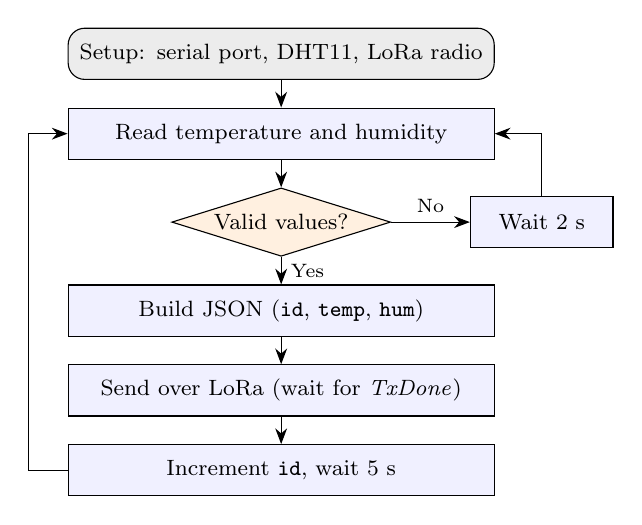
\begin{tikzpicture}[node distance=0.35cm and 1cm]
        \node[term] (start) {Setup: serial port, DHT11, LoRa radio};
        \node[proc, below=of start] (read) {Read temperature and humidity};
        \node[dec, below=of read] (valid) {Valid values?};
        \node[proc, right=of valid, text width=1.6cm] (wait2) {Wait 2~s};
        \node[proc, below=of valid] (json) {Build JSON (\texttt{id}, \texttt{temp}, \texttt{hum})};
        \node[proc, below=of json] (send) {Send over LoRa (wait for \emph{TxDone})};
        \node[proc, below=of send] (inc) {Increment \texttt{id}, wait 5~s};

        \coordinate (L) at ([xshift=-0.5cm]read.west);

        \draw[arr] (start) -- (read);
        \draw[arr] (read) -- (valid);
        \draw[arr] (valid) -- node[lbl, above] {No} (wait2);
        \draw[arr] (wait2) |- (read.east);
        \draw[arr] (valid) -- node[lbl, right] {Yes} (json);
        \draw[arr] (json) -- (send);
        \draw[arr] (send) -- (inc);
        \draw[arr] (inc.west) -- (inc.west -| L) -- (L) -- (read.west);
    \end{tikzpicture}
    \caption{Flowchart of the TX node.}
    \label{fig:tx-flow}
\end{figure}

% =====================================================================
\section{RX node}
\label{sec:rx}
% =====================================================================

The RX node bridges the LoRa link and the MQTT chain of Activity 1: it waits for the packets of the TX node, extracts the temperature and humidity and republishes them to the Mosquitto broker. It is built in its own environment (\texttt{env:rx}), reuses the \texttt{WiFiManager} and \texttt{MqttPublisher} classes of Activity 1 and adds the LoRa functions of Section~\ref{sec:lora-config}.

\paragraph{Initialisation.} \texttt{setup()} starts the WiFi manager and configures the radio with \texttt{LoRaIOT\_setup(LoRaConfig())}, the same call used by the TX node, so both boards share the same radio configuration. Then \texttt{LoRa.receive()} puts the radio in continuous receive mode; without it, the module would not listen and no packet would ever be detected.

\paragraph{Interrupt-driven reception.} During \texttt{LoRaIOT\_setup()}, \texttt{attachInterrupt()} associates the DIO0 pin of the radio, which rises when a complete packet is received, with \texttt{onLoRaRxIRQ()}:

\begin{lstlisting}[style=arduino]
extern volatile bool rxFlag;

void IRAM_ATTR onLoRaRxIRQ()
{
    rxFlag = true;   // only signal that a packet has arrived
}
\end{lstlisting}

The routine only raises a flag, since interrupt routines must be as short as possible. The flag is \texttt{volatile} because it is modified from the interrupt and read from \texttt{loop()}, and \texttt{IRAM\_ATTR} keeps the routine in the internal RAM of the ESP32. The heavy work is done in the main loop.

\paragraph{Main loop.} On every iteration, \texttt{loop()} updates the WiFi manager, keeps the MQTT connection alive as in Activity 1 and, if \texttt{rxFlag} is set, clears it and reads the packet with \texttt{LoRaIOT\_receive()}. This function reads the packet byte by byte with \texttt{LoRa.parsePacket()} and \texttt{LoRa.read()}, prints it with its RSSI and puts the radio back into receive mode. Unlike in Activity 1, publication is no longer periodic: the publishing rate is set by the TX node. Figure~\ref{fig:rx-flow} summarises the whole loop, including the interrupt that raises the flag.

\begin{figure}[htbp]
    \centering
    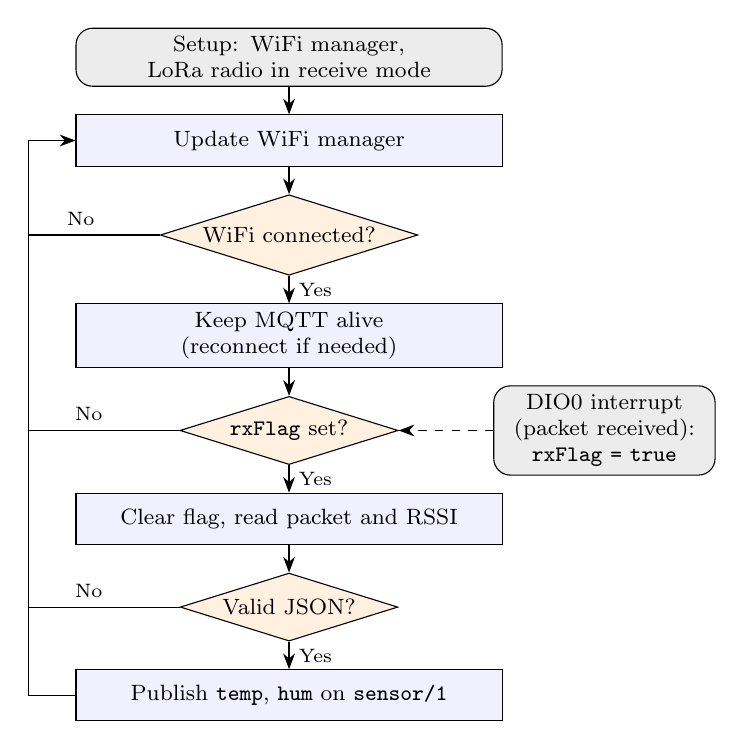
\begin{tikzpicture}[node distance=0.35cm and 1.2cm]
        \node[term] (start) {Setup: WiFi manager, LoRa radio in receive mode};
        \node[proc, below=of start] (wifi) {Update WiFi manager};
        \node[dec, below=of wifi] (wok) {WiFi connected?};
        \node[proc, below=of wok] (mqtt) {Keep MQTT alive\\ (reconnect if needed)};
        \node[dec, below=of mqtt] (flag) {\texttt{rxFlag} set?};
        \node[proc, below=of flag] (rd) {Clear flag, read packet and RSSI};
        \node[dec, below=of rd] (parse) {Valid JSON?};
        \node[proc, below=of parse] (pub) {Publish \texttt{temp}, \texttt{hum} on \texttt{sensor/1}};
        \node[term, right=of flag, text width=2.6cm] (isr) {DIO0 interrupt (packet received): \texttt{rxFlag = true}};

        \coordinate (L) at ([xshift=-0.6cm]wifi.west);

        \draw[arr] (start) -- (wifi);
        \draw[arr] (wifi) -- (wok);
        \draw[arr] (wok) -- node[lbl, right] {Yes} (mqtt);
        \draw[arr] (mqtt) -- (flag);
        \draw[arr] (flag) -- node[lbl, right] {Yes} (rd);
        \draw[arr] (rd) -- (parse);
        \draw[arr] (parse) -- node[lbl, right] {Yes} (pub);

        \draw (wok.west)   -- node[lbl, above, pos=0.6] {No} (wok.west -| L);
        \draw (flag.west)  -- node[lbl, above, pos=0.6] {No} (flag.west -| L);
        \draw (parse.west) -- node[lbl, above, pos=0.6] {No} (parse.west -| L);
        \draw (pub.west)   -- (pub.west -| L);
        \draw[arr] (pub.west -| L) -- (L) -- (wifi.west);

        \draw[arr, dashed] (isr) -- (flag);
    \end{tikzpicture}
    \caption{Flowchart of the RX node. The dashed arrow is the interrupt, which runs asynchronously and only raises the flag checked by the main loop.}
    \label{fig:rx-flow}
\end{figure}

\paragraph{From LoRa to MQTT.} \texttt{publishReading()} deserialises the received JSON with ArduinoJson, discards the packet if parsing fails, keeps only the temperature and humidity and publishes them with the same fields as in Activity 1:

\begin{lstlisting}[style=arduino]
StaticJsonDocument<200> doc;
DeserializationError error = deserializeJson(doc, message);

if (error) return false;
float temperature = doc["temp"];
float humidity = doc["hum"];

publisher.addField("temp", temperature);
publisher.addField("hum", humidity);
publisher.publish(topic, retained);
\end{lstlisting}

%Since the message format and the topic (\texttt{sensor/1}) are the same as in Activity 1, the WiFi and MQTT handling, the broker and the Dash/Plotly dashboard remain unchanged: the dashboard cannot tell whether the data comes from a local sensor or from a remote one over LoRa.

\paragraph{Reused components from Activity 1.} The WiFi connection (the non-blocking \texttt{WiFiManager} state machine), the MQTT client (\texttt{MqttPublisher}, with automatic reconnection and JSON serialisation), the Mosquitto broker running in Docker and the Dash/Plotly dashboard are not new in this activity: they were developed by Marcos García and Aarón Alcalá in their Activity 1 and are reused here without modification, so they are not described again in this report. The work specific to Activity 2 on the RX node is limited to the LoRa reception and the conversion of the received packets into MQTT messages.

% =====================================================================
\section{Experiments}
\label{sec:experiments}
% =====================================================================

\subsection{Transmission power vs.\ energy consumption and signal strength}
\label{sec:exp-txpower}

This experiment evaluates how the transmission power affects the signal strength at the receiver and the energy needed to send each packet.

\subsubsection{Test procedure}

A dedicated test program (\texttt{test/test\_tx\_power}) runs on the transmitter. It initialises the radio with the normal configuration (SF7, 250~kHz, CR 4/5, 868~MHz) and, for each power level in $\{2, 5, 8, 11, 14, 17, 20\}$~dBm, sends 10 packets 500~ms apart, such as \texttt{\{"test":"tx\_power","power":14,"seq":3\}}. For each packet it measures the duration of \texttt{LoRaIOT\_send()}, which, since \texttt{endPacket()} blocks until \emph{TxDone}, is the time on air plus a small SPI overhead. The receiver runs its normal firmware and logs the RSSI of every packet. Five sweeps were recorded, with both Heltec WiFi LoRa 32 V2 boards on a table 1~m apart with line of sight.

The transmitter was powered from a laboratory supply at 5~V, whose current display was recorded on video. The energy per packet is
\begin{equation}
    E_{\text{packet}} = V \cdot I \cdot t_{\text{air}},
    \label{eq:energy}
\end{equation}
computed for the whole board with the current during transmission, $I_{\text{TX}}$, and for the radio alone with the increase over the idle current, $\Delta I = I_{\text{TX}} - I_{\text{idle}}$. The time on air depends only on SF, BW, CR, preamble and payload, not on the power (Eq.~\eqref{eq:toa}); for the 37--38-byte test packets it is about 41~ms.

\subsubsection{Results and discussion}

The measured time on air was 42.0--42.1~ms at every power level, about 1~ms above the theoretical value because of the SPI write and the \emph{TxDone} detection. In total, 230 packets were received (the receiver was restarted once during the second sweep). Table~\ref{tab:txpower} and Figure~\ref{fig:txpower-results} summarise the results; the idle current was 42~mA.

\begin{table}[htbp]
    \centering
    \small
    \begin{tabular}{@{}ccccccc@{}}
        \toprule
        \textbf{Power} & \textbf{Packets} & \textbf{RSSI}  &
        $I_{\text{TX}}$ & $\Delta I$ & \textbf{E (board)} & \textbf{E (radio)} \\
        (dBm) & & (dBm)  & (mA) & (mA) & (mJ) & (mJ) \\
        \midrule
        2  & 30 & $-47.4$ & 50 & 8  & 10.53 & 1.68 \\
        5  & 40 & $-44.8$ & 51 & 9  & 10.74 & 1.89 \\
        8  & 29 & $-41.3$ & 52 & 10 & 10.95 & 2.11 \\
        11 & 37 & $-39.2$ & 54 & 12 & 11.37 & 2.53 \\
        14 & 30 & $-35.9$ & 57 & 15 & 12.00 & 3.16 \\
        17 & 29 & $-33.0$ & 61 & 19 & 12.84 & 4.00 \\
        20 & 30 & $-30.9$ & 65 & 23 & 13.68 & 4.84 \\
        \bottomrule
    \end{tabular}
    \caption{RSSI at the receiver and current and energy per packet at the transmitter (5~V, $t_{\text{air}} = 42.1$~ms).}
    \label{tab:txpower}
\end{table}

\begin{figure}[htbp]
    \centering
\pgfplotsset{
        pwplot/.style={
            width=0.48\textwidth, height=4.8cm,
            xlabel={TX power (dBm)}, xtick={2,5,8,11,14,17,20},
            xmin=0, xmax=22, grid=major,
            legend style={font=\scriptsize}, legend cell align=left,
        },
    }
\begin{tikzpicture}
\begin{axis}[pwplot, ylabel={RSSI (dBm)},
                     title={(a) Mean RSSI}]
\addplot[mark=*, blue, error bars/.cd, y dir=both, y explicit]
            coordinates {
                (2,-47.4)
                (5,-44.8)
                (8,-41.3)
                (11,-39.2)
                (14,-35.9)
                (17,-33.0)
                (20,-30.9)
            };
\end{axis}
\end{tikzpicture}
\hfill
\begin{tikzpicture}
\begin{axis}[pwplot, ylabel={Energy per packet (mJ)}, ymin=0, ymax=20,
                     title={(b) Energy per packet},
                     legend style={at={(0.03,0.8)}, anchor=west}]
\addplot[mark=square*, red] coordinates {
                (2,10.53) (5,10.74) (8,10.95) (11,11.37) (14,12.00) (17,12.84) (20,13.68)
            };
\addlegendentry{Board}
\addplot[mark=triangle*, orange] coordinates {
                (2,1.68) (5,1.89) (8,2.11) (11,2.53) (14,3.16) (17,4.00) (20,4.84)
            };
\addlegendentry{Radio ($\Delta I$)}
\end{axis}
\end{tikzpicture}
\caption{Mean RSSI at the receiver with its standard deviation (a) and energy per packet at the transmitter (b) as a function of the transmission power.}
\label{fig:txpower-results}
\end{figure}


The RSSI grows almost linearly with the power (linear fit slope of 0.93~dB/dB, close to the ideal 1~dB/dB), with no saturation even at 20~dBm. The spread between sweeps is larger than within a sweep, which points to changes in the environment (people moving, boards touched) rather than random noise. Practically no packets were lost, and even at 2~dBm the RSSI is more than 70~dB above the SX1276 sensitivity for SF7/250~kHz ($-120$~dBm, Table~10 of~\cite{sx1276}).

Since the time on air is constant, the energy follows the current: the radio needs 1.7~mJ per packet at 2~dBm and 4.8~mJ at 20~dBm, about 2.9 times more. For the whole board the increase is smaller (10.5 to 13.7~mJ), because most of the energy is consumed by the ESP32. These currents should be read as a trend: a 42~ms transmission is shorter than the refresh time of the supply display, which partly averages it with the idle current, and the datasheet gives much higher values for the radio alone (87~mA at 17~dBm and 120~mA at 20~dBm, Table~6 of~\cite{sx1276}). An oscilloscope with a shunt resistor would be needed to measure the real peak.

\subsection{Bandwidth and data rate}
\label{sec:exp-bw}

This experiment quantifies the trade-off between transmission speed and range when the bandwidth and the spreading factor are changed. Each LoRa symbol lasts $T_{\text{sym}} = 2^{SF}/BW$, and the time on air of a packet is
\begin{equation}
    t_{\text{air}} = \left(n_{\text{pre}} + 4.25 + n_{\text{pl}}\right) T_{\text{sym}},
    \label{eq:toa}
\end{equation}
where $n_{\text{pre}} = 8$ is the preamble and $n_{\text{pl}}$ the number of payload symbols given by the SX1276 datasheet~\cite{sx1276}. A slower configuration is more sensitive: the minimum SNR needed to demodulate, $SNR_{\min}$, goes from $-7.5$~dB at SF7 to $-20$~dB at SF12 (about 2.5~dB per SF step), and halving $BW$ gains another 3~dB, from $-118.5$~dBm at SF7/500~kHz to $-137$~dBm at SF12/125~kHz. In exchange, the 1\,\% EU868 duty cycle forces an off-time of $99\,t_{\text{air}}$ after each packet.

\subsubsection{Experimental setup}

A dedicated firmware (\texttt{test/range\_speed\_balance\_bw}) sweeps the nine combinations of $BW \in \{125, 250, 500\}$~kHz and $SF \in \{7, 9, 12\}$. Since two boards with different configurations cannot communicate, the change cannot be negotiated over LoRa: both boards synchronise their clocks through WiFi and NTP at boot and switch configuration in time windows aligned to the wall clock. In each window the transmitter sends 10 packets with a sequence number and a timestamp (27~bytes), spaced $t_{\text{air}}/0.01$ (minimum 5~s) to respect the duty cycle, so a full cycle takes about 57~min. The transmitter logs the measured and theoretical time on air, and the receiver the RSSI, SNR and $\Delta t = t_{\text{rx}} - t_{\text{tx}}$. The boards were placed indoors, about 5~m apart.

\subsubsection{Results and discussion}

Table~\ref{tab:bw-results} and Figure~\ref{fig:bw-results} show one complete cycle (90 packets).

\begin{table}[htbp]
    \centering
    \small
    \setlength{\tabcolsep}{4.5pt}
    \begin{tabular}{@{}cc rr r r r r c@{}}
        \toprule
        \textbf{BW} & \textbf{SF} & \multicolumn{2}{c}{$\boldsymbol{t_{\text{air}}}$ \textbf{(ms)}} & $\boldsymbol{\Delta t}$ & $\boldsymbol{R_{\text{eff}}}$  & \textbf{RSSI} & \textbf{SNR} & \textbf{Received} \\
        \cmidrule(lr){3-4}
        (kHz) & & Theory & Measured & (ms) & (kbps)  & (dBm) & (dB) & (of 10) \\
        \midrule
        125 & 7  & 66.8   & 67.6   & 78.6   & 3.20    & $-49.4$ & 9.9  & 10 \\
        125 & 9  & 226.3  & 227.1  & 238.3  & 0.95    & $-51.9$ & 12.7 & 10 \\
        125 & 12 & 1646.6 & 1647.4 & 1716.7 & 0.13    & $-46.9$ & 9.1  & 10 \\
        \midrule
        250 & 7  & 33.4   & 34.2   & 64.2   & 6.32    & $-43.6$ & 10.1 & 10 \\
        250 & 9  & 113.2  & 114.0  & 144.1  & 1.89    & $-49.5$ & 11.9 & 10 \\
        250 & 12 & 741.4  & 742.2  & 779.1  & 0.29    & $-47.3$ & 9.9  & 10 \\
        \midrule
        500 & 7  & 16.7   & 17.5   & 34.4   & 12.34  & $-40.3$ & 5.5  & 10 \\
        500 & 9  & 56.6   & 57.4   & 74.0   & 3.76   & $-46.4$ & 7.8  & 10 \\
        500 & 12 & 370.7  & 371.5  & 392.0  & 0.58   & $-47.8$ & 7.4  & 10 \\
        \bottomrule
    \end{tabular}
    \caption{Results of the bandwidth and spreading factor sweep (averages of 10 packets, $R_{\text{eff}} = 8PL/t_{\text{air}}$).}
    \label{tab:bw-results}
\end{table}

\begin{figure}[htbp]
    \centering
    \pgfplotsset{
        bwplot/.style={
            width=0.48\textwidth, height=4.8cm,
            xlabel={Spreading factor}, xtick={7,9,12},
            xmin=6.5, xmax=12.5, grid=major,
            legend style={font=\scriptsize}, legend cell align=left,
        },
    }
    \begin{tikzpicture}
        \begin{axis}[bwplot, ymode=log, ylabel={$t_{\text{air}}$ (ms)},
                     title={(a) Measured time on air}, legend pos=north west]
            \addplot[mark=*, blue] coordinates {(7,67.6) (9,227.1) (12,1647.4)};
            \addlegendentry{125 kHz}
            \addplot[mark=square*, red] coordinates {(7,34.2) (9,114.0) (12,742.2)};
            \addlegendentry{250 kHz}
            \addplot[mark=triangle*, green!50!black] coordinates {(7,17.5) (9,57.4) (12,371.5)};
            \addlegendentry{500 kHz}
        \end{axis}
    \end{tikzpicture}
    \hfill
    \begin{tikzpicture}
        \begin{axis}[bwplot, ymode=log, ylabel={$\Delta t$ (ms)},
                     title={(b) Latency $\Delta t$}]
            \addplot[mark=*, blue] coordinates {(7,78.6) (9,238.3) (12,1716.7)};
            \addplot[mark=square*, red] coordinates {(7,64.2) (9,144.1) (12,779.1)};
            \addplot[mark=triangle*, green!50!black] coordinates {(7,34.4) (9,74.0) (12,392.0)};
        \end{axis}
    \end{tikzpicture}

    \medskip
    \begin{tikzpicture}
        \begin{axis}[bwplot, ymode=log, ylabel={$R_{\text{eff}}$ (kbps)},
                     title={(c) Effective data rate}]
            \addplot[mark=*, blue] coordinates {(7,3.20) (9,0.951) (12,0.131)};
            \addplot[mark=square*, red] coordinates {(7,6.32) (9,1.89) (12,0.291)};
            \addplot[mark=triangle*, green!50!black] coordinates {(7,12.34) (9,3.76) (12,0.581)};
        \end{axis}
    \end{tikzpicture}
    \hfill
    \begin{tikzpicture}
        \begin{axis}[bwplot, ylabel={SNR (dB)}, ymin=-25, ymax=20,
                     title={(d) Average SNR}]
            \addplot[mark=*, blue] coordinates {(7,9.9) (9,12.7) (12,9.1)};
            \addplot[mark=square*, red] coordinates {(7,10.1) (9,11.9) (12,9.9)};
            \addplot[mark=triangle*, green!50!black] coordinates {(7,5.5) (9,7.8) (12,7.4)};
            \addplot[black, dashed, mark=none] coordinates {(7,-7.5) (9,-12.5) (12,-20)}
                node[pos=0.5, anchor=south west, font=\scriptsize] {$SNR_{\min}$};
        \end{axis}
    \end{tikzpicture}
    \caption{Results of the bandwidth and spreading factor sweep: measured time on air at the transmitter (a), latency $\Delta t$ measured at the receiver (b), effective data rate (c) and average SNR with the demodulation limit $SNR_{\min}$ (d).}
    \label{fig:bw-results}
\end{figure}

All 90 packets were received, so no configuration reached its range limit at this distance. Packets from other groups using the same radio settings were also decoded (and discarded for lacking a valid timestamp), which confirms that the sync word does not isolate the network.

The measured time on air matches Eq.~\eqref{eq:toa} with a constant overhead of 0.8~ms: doubling $BW$ halves it, and the effective data rate ranges from 12.3~kbps (SF7/500~kHz) to 0.13~kbps (SF12/125~kHz), a factor of 94. $\Delta t$ is 11--69~ms longer than $t_{\text{air}}$, mostly because of the drift between the clocks of both boards (about 13~ppm), so the time on air measured at the transmitter is the reliable speed metric.

The RSSI stays between $-40$ and $-52$~dBm with no trend, as expected. The reported SNR (5--13~dB) is far below the value expected from the RSSI, which indicates that the SX1276 SNR estimate saturates for strong signals; even so, the 500~kHz configurations show 2.5--4.6~dB less SNR than the 250~kHz ones, and the margin over $SNR_{\min}$ grows from 13--18~dB at SF7 to 27--30~dB at SF12.

\subsection{Quality of Service: packet loss vs.\ distance}
\label{sec:exp-qos}

This experiment evaluates how the signal strength and the packet delivery degrade as the distance between both nodes increases. The RSSI is expected to follow the log-distance path loss model,
\begin{equation}
    RSSI(d) = RSSI(d_0) - 10\,n\log_{10}\frac{d}{d_0} + X_\sigma,
    \label{eq:pathloss}
\end{equation}
where $n$ is the path loss exponent (2 in free space, 2.7--4 with obstacles) and $X_\sigma$ a random fading term. Packets are lost only when the RSSI approaches the sensitivity, about $-121.5$~dBm at SF7/250~kHz.

\subsubsection{Experimental setup}

The boards ran the normal TX and RX firmware, each connected to a laptop logging the sent and received packets. The receiver stayed fixed on the third floor of the university building, and the transmitter was carried along the corridor and stopped at approximately 1, 12, 27, 40, 57 and 65~m, sending 8--10 readings at each position, with doors and columns between both nodes. The transmitter was reset at each position, so lost packets appear as gaps in the \texttt{id} sequence. An extra measurement was taken about 60~m away and one floor below, behind several walls.

\subsubsection{Results and discussion}

\begin{table}[htbp]
    \centering
    \small
    \begin{tabular}{@{}cccccc@{}}
        \toprule
        \textbf{Distance} & \textbf{Sent} & \textbf{Received} & \textbf{Loss} & \textbf{Avg.\ RSSI} & \textbf{RSSI range} \\
        (m) & & & (\%) & (dBm) & (dBm) \\
        \midrule
        1  & 8  & 8  & 0    & $-39.0$ & $-57$ to $-31$ \\
        12 & 8  & 8  & 0    & $-52.3$ & $-61$ to $-46$ \\
        27 & 9  & 9  & 0    & $-63.2$ & $-71$ to $-53$ \\
        40 & 9  & 9  & 0    & $-72.9$ & $-84$ to $-62$ \\
        57 & 8  & 8  & 0    & $-73.5$ & $-85$ to $-65$ \\
        65 & 10 & 10 & 0    & $-81.4$ & $-93$ to $-69$ \\
        \midrule
        60* & 6 & 5 & 16.7 & $-88.8$ & $-92$ to $-87$ \\
        \bottomrule
    \end{tabular}
    \caption{Packet loss and RSSI at different distances (SF7, 250~kHz, 20~dBm). *One floor below, behind several walls.}
    \label{tab:qos-results}
\end{table}

\begin{figure}[htbp]
    \centering
    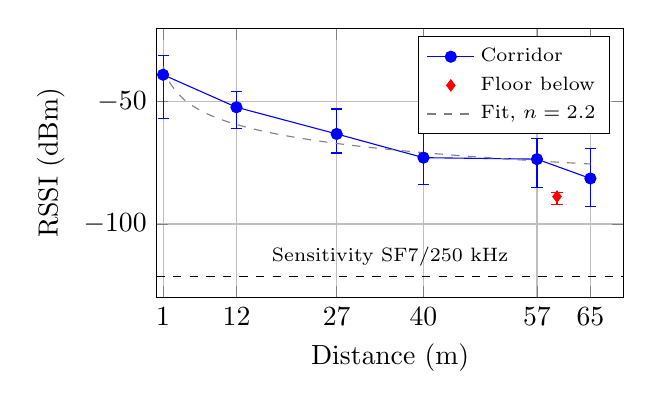
\begin{tikzpicture}
        \begin{axis}[
            width=0.62\textwidth, height=5cm,
            xlabel={Distance (m)}, ylabel={RSSI (dBm)},
            xtick={1,12,27,40,57,65}, xmin=0, xmax=70, ymin=-130, ymax=-20,
            grid=major,
            legend pos=north east, legend style={font=\scriptsize}, legend cell align=left
        ]
            \addplot[mark=*, blue, error bars/.cd, y dir=both, y explicit] coordinates {
                (1,-39.0)  += (0,8.0)  -= (0,18.0)
                (12,-52.3) += (0,6.3)  -= (0,8.7)
                (27,-63.2) += (0,10.2) -= (0,7.8)
                (40,-72.9) += (0,10.9) -= (0,11.1)
                (57,-73.5) += (0,8.5)  -= (0,11.5)
                (65,-81.4) += (0,12.4) -= (0,11.6)
            };
            \addlegendentry{Corridor}
            \addplot[only marks, mark=diamond*, red, error bars/.cd, y dir=both, y explicit] coordinates {
                (60,-88.8) += (0,1.8) -= (0,3.2)
            };
            \addlegendentry{Floor below}
            \addplot[gray, dashed, domain=1:65, samples=60] {-35.6 - 22.0*log10(x)};
            \addlegendentry{Fit, $n = 2.2$}
            \addplot[black, dashed, mark=none, forget plot] coordinates {(0,-121.5) (70,-121.5)}
                node[pos=0.5, anchor=south, font=\scriptsize] {Sensitivity SF7/250~kHz};
        \end{axis}
    \end{tikzpicture}
    \caption{RSSI as a function of the distance. Error bars show the minimum and maximum RSSI at each position and the dashed grey line is the least-squares fit of Eq.~\eqref{eq:pathloss}.}
    \label{fig:qos-results}
\end{figure}

Table~\ref{tab:qos-results} and Figure~\ref{fig:qos-results} summarise the results. The RSSI decreased from $-39.0$~dBm at 1~m to $-81.4$~dBm at 65~m, with a spread of 15--26~dB at each position. A least-squares fit gives $n = 2.2$ with $RSSI(1~\text{m}) = -35.6$~dBm (RMS error of 4.4~dB), only slightly above free space: the corridor probably guides part of the energy, and the doors and columns appear mainly as large fluctuations of $X_\sigma$.

No packet was lost along the corridor, since even the weakest packet ($-93$~dBm) kept a margin of about 28~dB over the sensitivity. The only loss (one of six packets) occurred one floor below, where the average RSSI dropped to $-88.8$~dBm; as the received packets were still about 30~dB above the sensitivity, it was more likely caused by a deep fade or interference than by the average path loss, although six packets are not enough for a significant PDR estimate.

% =====================================================================
\section{Answers to Guiding Questions}
\label{sec:questions}
% =====================================================================

\begin{enumerate}[label=\textbf{Q\arabic*.}, leftmargin=*]
    \item \textbf{How does LoRa compare to Wi-Fi and Bluetooth in terms of range and power consumption?}

    LoRa offers a much longer range than Wi-Fi and Bluetooth, from hundreds of metres to several kilometres under suitable conditions, while keeping a low average power consumption. The price is a low data rate, so it is only suitable for small messages. Wi-Fi is much faster, but it has a shorter range, needs an access point and generally consumes more energy, while Bluetooth also consumes little but only works at short distances (the exact figures depend on the hardware, the Bluetooth version and the environment). LoRa fits our project because the boards only exchange a small sensor reading every few seconds and no network infrastructure is needed.

    \item \textbf{What are the trade-offs of using lower data rates in LoRa transmission?}

    Lowering the data rate (by increasing the spreading factor or reducing the bandwidth) makes the signal easier for the receiver to detect, which increases the sensitivity and the potential range. The price is a longer time on air: the radio stays on for longer, so each message costs more energy, the shared channel is occupied for longer and the probability of collisions grows, the regulations allow fewer messages per hour and the data arrives with more delay. Therefore, a lower data rate does not necessarily mean a lower consumption. In our case, SF7 with 250~kHz keeps the transmissions short, which is appropriate for small sensor messages as long as the receiver decodes them reliably; a higher spreading factor would only be needed for more range.

    \item \textbf{How does increasing transmission power affect battery life and interference?}

    A higher transmission power improves the received signal strength and can extend the range, but the radio draws more current while transmitting, so the battery lasts less (the consumption does not grow in the same proportion as the radiated power, since it also depends on the efficiency of the radio). It also increases the interference with other devices sharing the same frequencies and, if the boards are very close, it can overload the receiver. The best strategy is therefore to use the minimum power that keeps a reliable link, and the final setting must comply with the radio regulations. In our project, the RSSI measurements and the packet reception of the power experiment (Section~\ref{sec:exp-txpower}) help to find it.
\end{enumerate}

% =====================================================================
\section{Discussion and conclusions}
\label{sec:conclusions}
% =====================================================================

The weather station works end to end over LoRa: the TX node reads the DHT11 and sends each reading without any network infrastructure, and the RX node republishes it in the same MQTT format as in Activity~1, so the broker and the dashboard did not need any change.

In the conditions we tested, the link was never close to its limit: all 90 packets of the bandwidth sweep were received, and no packet was lost along the 65~m corridor, where the weakest packet arrived at $-93$~dBm. Making the link more robust therefore brought no benefit in our scenario, only costs. Raising the power from 2 to 20~dBm improved the RSSI by 16.5~dB but almost tripled the energy of the radio per packet (from 1.7 to 4.8~mJ), and moving from SF7 to SF12 at 250~kHz increased the time on air from 34 to 742~ms. For this reason, SF7/250~kHz with a low transmission power is a suitable configuration for the weather station.

The power experiment also showed that the radio is not the main consumer: at every level, most of the energy per packet was spent by the ESP32, which stays active between readings. For a battery-powered station, putting the microcontroller in deep sleep between transmissions would save much more energy than tuning the radio.

The results also have some limitations. The current was read from the display of the power supply, so the energy values show a trend rather than the exact consumption, and all the tests were carried out indoors at distances of up to 65~m, so the range limit of the link was not reached. In addition, packets from other groups were decoded with our settings, which shows that the sync word does not isolate the network. Future work should include current measurements with an oscilloscope, outdoor tests at longer distances and encryption of the payload.

\begin{thebibliography}{9}
    \bibitem{sx1276} Semtech Corporation, \emph{SX1276/77/78/79 -- 137~MHz to 1020~MHz Low Power Long Range Transceiver}, datasheet, Rev.~7, May 2020.
\end{thebibliography}

\end{document}